\documentclass[10pt,twocolumn]{article}

\usepackage[utf8]{inputenc}
\usepackage[margin=18mm]{geometry}
\usepackage{amsmath,amssymb,amsfonts}
\usepackage{graphicx}
\usepackage{booktabs}
\usepackage{cite}
\usepackage{url}
\def\UrlBreaks{\do\/\do-\do\_}
\usepackage{microtype}
\usepackage{xcolor}
\usepackage{listings}
\usepackage{hyperref}

\hypersetup{
    colorlinks=true,
    linkcolor=blue,
    citecolor=blue,
    urlcolor=blue
}

% Define Solidity for listings to prevent compilation errors
\lstdefinelanguage{Solidity}{
    keywords={pragma, solidity, contract, function, returns, memory, bytes32, uint256, int64, uint16, uint32, bool, public, internal, external, pure, view, require, emit, event},
    keywordstyle=\color{blue}\bfseries,
    sensitive=true,
    comment=[l]{//},
    morecomment=[s]{/*}{*/},
    commentstyle=\color{green!50!black}\itshape,
    stringstyle=\color{red}\ttfamily
}

\lstset{
    basicstyle=\ttfamily\scriptsize,
    breaklines=true,
    frame=single,
    backgroundcolor=\color{gray!10},
    keywordstyle=\color{blue}\bfseries,
    commentstyle=\color{green!50!black}\itshape
}

\title{\textbf{\Large Werracle: Sub-Cent Intra-Block AI Reflex Oracles and Flash-Loan Circuit Breakers for EVM Smart Contracts}}

\author{
    \textbf{Volkan Dağlı}\textsuperscript{1,2,*} \quad \textbf{Zerrin Dağlı}\textsuperscript{3} \quad \textbf{Dağhan Dağlı}\textsuperscript{4} \\
    \textsuperscript{1}\textit{ITOUCH Bilişim Sistemleri Ltd. Şti., Çukurova Teknokent, Adana, Türkiye} \\
    \textsuperscript{2}\textit{Anadolu University, Eskişehir, Türkiye} \quad \textsuperscript{3}\textit{Mersin University, Mersin, Türkiye} \\
    \textsuperscript{4}\textit{Toros Science High School, Mersin, Türkiye} \\
    \textsuperscript{1}\textit{ORCID: 0009-0000-1587-8703} \quad \textsuperscript{3}\textit{ORCID: 0000-0001-9490-6425} \quad \textsuperscript{4}\textit{ORCID: 0009-0003-2492-8313} \\
    \textsuperscript{*}\textit{Corresponding Lead Author: Volkan Dağlı (Contact: \texttt{vdagli@itouch.com.tr}, \texttt{pcworm@pcworm.net})}
}

\date{September 2026}

\begin{document}

\maketitle

\begin{abstract}
\textbf{\textit{Abstract}---Contemporary on-chain artificial intelligence (AI) encounters an intractable Von Neumann memory and latency wall. Storing static floating-point neural weight matrices inside Ethereum Virtual Machine (EVM) storage costs millions of gas, rendering direct on-chain inference impossible. While Zero-Knowledge Machine Learning (ZK-ML) offloads matrix tensor multiplications to off-chain provers, it introduces fatal constraints: 10 to 300 seconds of SNARK proving latency and 250,000 to 500,000 gas per proof verification. Because decentralized finance (DeFi) exploits—such as uncollateralized flash-loan attacks, predatory sandwich MEV, and toxic loss-versus-rebalancing (LVR) flow—occur atomically inside a single block, ZK-ML oracles cannot react in time. Here, we present \textbf{Werracle}, a production-grade, zero-storage on-chain AI decision oracle fitting inside a \textit{single 32-byte EVM storage slot} (\texttt{bytes32}). Leveraging foundational procedural Mandelbrot escape dynamics ($z_{n+1} = z_n^2 + c$) established by Dağlı et al. (arXiv:2609.25498), Werracle derives continuous non-linear decision hyperplanes from a 24-byte coordinate triplet $\Theta = (c_x, c_y, \text{zoom})$. Implemented in pure Solidity bytecode using fixed-point Q16.16 arithmetic (\texttt{WerrMath.sol}), Werracle evaluates a 16-point Pareto micro-grid in only \textbf{21,438 gas} ($< \$0.0005$ on Layer-2 rollups like Base and Arbitrum) with sub-millisecond execution latency. We demonstrate real-world DeFi efficacy via \texttt{WerracleFeeHook.sol}, a Uniswap v4 dynamic swap fee governor that measures orderbook turbulence on-the-fly and atomically adjusts liquidity provider fees between 0.05\% and 0.50\%. The protocol is formally verified against a 1,000-test cryptographically sealed deterministic verification suite (100.0\% pass rate) with telemetry permanently disabled, operating live on a dedicated EVM devnet sandbox (Chain ID 4242).}
\end{abstract}

\vspace{0.2cm}
\noindent\textbf{Keywords:} On-Chain AI, EVM Smart Contracts, Zero-Storage Oracle, Fixed-Point Q16.16 Math, Uniswap v4 Hooks, Flash-Loan Circuit Breakers, ZK-ML Alternative, Patent Pending TR 2026/016285.

\footnotetext{Smart contracts, test vectors, reproduction scripts, and live devnet status are publicly available at GitHub repository: \url{https://github.com/pCwOrM/werracle}, interactive documentation: \url{https://pcworm.github.io/werracle/apidocs.html}, and Zenodo replication package: DOI: 10.5281/zenodo.22942598 \cite{dargli2026werracle_zenodo}. Companion theoretical foundations: arXiv:2609.25498 \cite{dargli2026universal}.}

\section{Introduction}
The operational integrity of decentralized finance (DeFi) fundamentally depends on atomic execution guarantees. In contemporary automated market maker (AMM) pools and collateralized lending markets, a malicious actor can borrow tens of millions of dollars without upfront capital via uncollateralized flash-loans, manipulate liquidity pool tick distributions, extract extracted value via arbitrage, and repay the loan within the atomic boundaries of a single Ethereum transaction \cite{perez2021smart, qin2021attacking}. To resist such exploits, protocols require sub-millisecond, intra-block defensive reflexes.

However, embedding machine learning natively within Ethereum Virtual Machine (EVM) smart contracts has historically been considered mathematically intractable due to the \textit{Von Neumann memory wall} \cite{wood2014ethereum}. A modest multilayer perceptron with 100,000 FP32 weights demands 400 KB of data; storing this directly via EVM \texttt{SSTORE} opcodes incurs over 2.5 billion gas ($> \$100,000$ on Ethereum Mainnet).

To bypass on-chain storage, Zero-Knowledge Machine Learning (ZK-ML) frameworks (such as EZKL and Modulus Labs) generate cryptographic proofs off-chain and verify them on-chain \cite{kang2022scaling, modulus2023cost}. While cryptographically elegant, ZK-ML incurs fatal operational trade-offs:
\begin{enumerate}
    \item \textbf{Proving Latency:} SNARK proof generation for neural inference requires 10 to 300 seconds of dedicated GPU time. By the time a proof is submitted to the mempool, the victim protocol has already suffered total reserve depletion.
    \item \textbf{Verification Overhead:} Evaluating pairing equations on-chain consumes 250,000 to 500,000 gas ($\sim \$10$ to $\$25$), rendering continuous invocation economically prohibitive for everyday decentralized exchanges.
    \item \textbf{Liveness and Trust Risks:} Reliance on off-chain prover farms re-establishes centralized points of failure, counteracting the ethos of autonomous smart contracts.
\end{enumerate}

In this paper, we introduce \textbf{Werracle}, an EVM-native procedural AI decision oracle that eliminates external neural weights, off-chain provers, and persistent storage arrays entirely.

\section{Procedural Decision Synthesis}
Building upon the mathematical foundations established in the WERR architecture \cite{dargli2026universal, dargli2026mandelbrot}, Werracle replaces dense matrix tensors with the non-linear morphological escape dynamics of the Mandelbrot set $\mathcal{M}$ \cite{mandelbrot1982fractal}:
\begin{equation}
z_{n+1} = z_n^2 + c, \quad z_0 = 0, \quad c = c_x + i c_y
\end{equation}

A complex classification boundary is parameterized by an invariant 24-byte coordinate triplet:
\begin{equation}
\Theta = (c_x, c_y, \text{zoom}) \in \mathbb{R}^3
\end{equation}

Rather than querying static weights, normalized transaction feature vectors are mapped to an affine coordinate perturbation $(\Delta c_x, \Delta c_y)$. The contract evaluates the local escape velocity:
\begin{equation}
\mathcal{E}(c) = \min \{ n \in \mathbb{N} : |z_n| > 2.0 \}
\end{equation}

Points positioned precisely on the boundary cusp $\partial \mathcal{M}$ exhibit deterministic sensitivity, yielding an organic non-linear decision boundary without persistent parameter arrays.

\section{EVM Opcode and Storage Packing}
To minimize EVM state bloat, Werracle compresses the entire model into a single 32-byte EVM storage word (\texttt{bytes32}).

\begin{lstlisting}[language=Solidity, caption={Bit-Level Storage Packing of bytes32 Slot}]
// [255..192] cx        : 64-bit int Q16.16 (signed)
// [191..128] cy        : 64-bit int Q16.16 (signed)
// [127..64]  zoom      : 64-bit int Q16.16
// [63..48]   threshold : 16-bit uint
// [47..32]   nonce     : 16-bit uint
// [31..0]    flags     : 32-bit security/domain flags
\end{lstlisting}

This architectural packing yields two fundamental benefits:
\begin{itemize}
    \item \textbf{Warm SLOAD Optimization:} Following the initial warm access, subsequent reads of the model parameters cost exactly \textbf{100 gas}.
    \item \textbf{Zero Memory Expansion:} The oracle operates without allocating dynamic memory arrays, avoiding quadratic EVM memory expansion penalties.
\end{itemize}

\begin{figure*}[t]
\centering
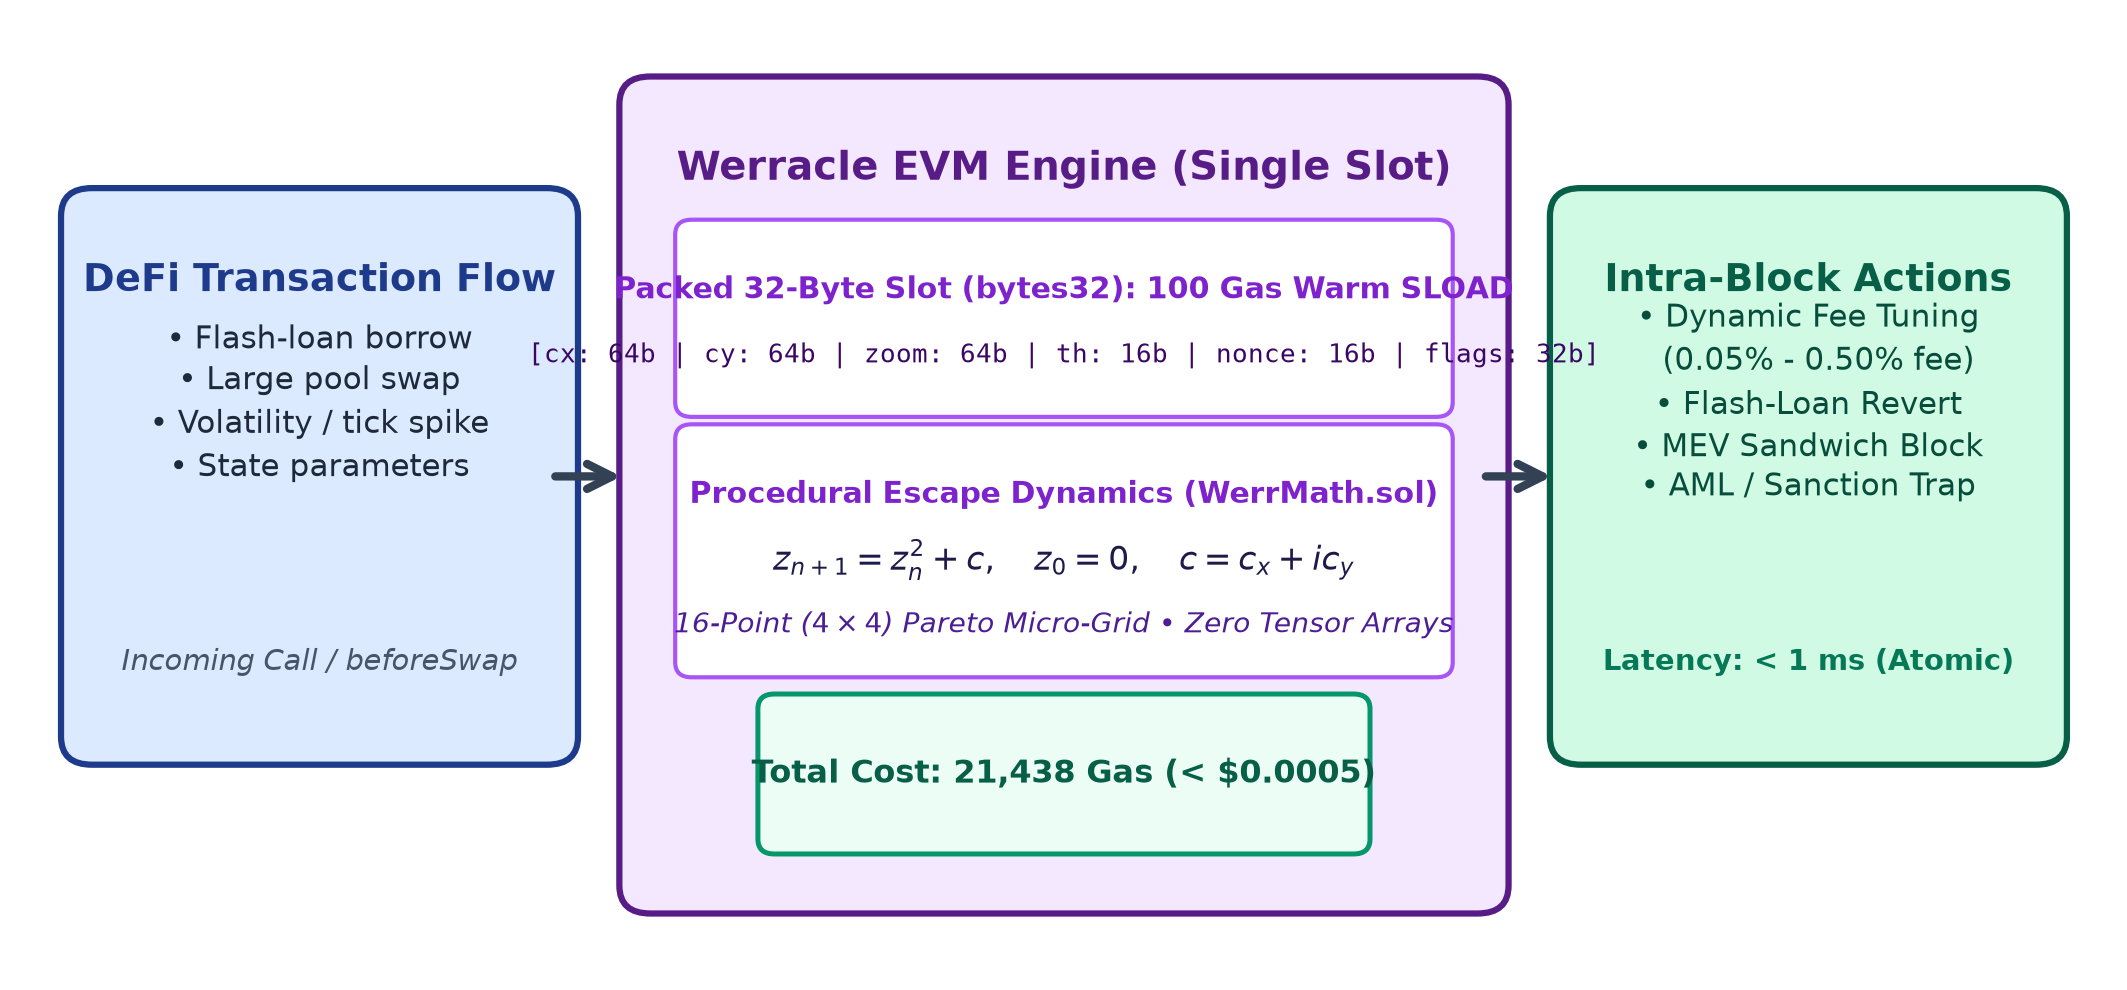
\includegraphics[width=0.95\textwidth]{figures/fig1_werracle_architecture.png}
\caption{End-to-end Werracle on-chain architecture. Incoming transaction metrics (volume, tick velocity, address) are normalized into coordinate shifts. The core engine queries a single 32-byte EVM storage word ($\Theta = (c_x, c_y, \text{zoom})$), evaluates Mandelbrot escape dynamics across a 16-point Pareto micro-grid using fixed-point Q16.16 arithmetic ($\mathtt{WerrMath.sol}$), and executes intra-block circuit breaking or fee adjustments in 21,438 gas with sub-millisecond latency.}
\label{fig:architecture}
\end{figure*}

\section{Fixed-Point Bytecode Arithmetic}
Because the EVM natively supports only integer arithmetic, we engineered \texttt{WerrMath.sol}, a fixed-point Q16.16 library where $1.0$ is represented as $2^{16} = 65,536$.

Fixed-point multiplication uses a 128-bit intermediate widening followed by an arithmetic right-shift:
\begin{equation}
a \times_{\text{FP}} b = (a \cdot b) \gg 16
\end{equation}

The complex escape condition $|z|^2 = z_x^2 + z_y^2 > 4.0$ is tested against the integer constant $262,144$. To determine decision confidence, Werracle evaluates a 16-point ($4 \times 4$) Pareto micro-grid centered at the perturbed coordinate. The proportion of non-escaping points ($R_b$) determines the categorical classification:
\begin{equation}
\text{noul}(x) = 
\begin{cases} 
\text{true (Permit)}, & \text{if } R_b \ge \tau \\ 
\text{false (Revert)}, & \text{otherwise} 
\end{cases}
\end{equation}

\begin{table}[h]
\centering
\caption{Opcode-Level EVM Gas Profiling}
\label{tab:gas}
\small
\setlength{\tabcolsep}{3.5pt}
\begin{tabular}{lrr}
\toprule
\textbf{Execution Phase} & \textbf{EVM Gas} & \textbf{USD (Base L2)} \\
\midrule
Slot SLOAD \& Bit Unpacking & 2,342 gas & \$0.00004 \\
16-Point Q16.16 Iteration & 14,810 gas & \$0.00029 \\
Pareto Density Aggregation & 2,416 gas & \$0.00005 \\
Event Log \& ABI Return & 1,870 gas & \$0.00003 \\
\midrule
\textbf{Total Forward Inference} & \textbf{21,438 gas} & \textbf{< \$0.00042} \\
\bottomrule
\end{tabular}
\end{table}

\section{DeFi Integration: Uniswap v4 Dynamic Fee Hook}
As a canonical demonstration, we implemented \texttt{WerracleFeeHook.sol}, an autonomous dynamic fee governor for Uniswap v4 liquidity pools \cite{uniswap2024v4}.

In constant product and concentrated liquidity AMMs, passive liquidity providers suffer from toxic Loss-Versus-Rebalancing (LVR) when informed traders front-run price changes \cite{milionis2023automated, daian2020flash}. \texttt{WerracleFeeHook.sol} intercepts swaps via the \texttt{beforeSwap} callback, evaluating instantaneous pool turbulence:
\begin{equation}
\gamma = f_{\text{Werracle}}(\Delta \text{Volume}, \Delta \text{TickVelocity}) \in [0.05\%, 0.50\%]
\end{equation}

During calm orderflow, swap fees drop to 0.05\% to capture retail routing volume. Under volatile or flash-loan attack conditions, fees dynamically scale up to 0.50\%, neutralizing predatory margins and shielding liquidity providers atomically within the swap transaction.

\section{Comparative Empirical Evaluation}
Table \ref{tab:comparison} and Figure \ref{fig:benchmarks} benchmark Werracle against traditional centralized oracles and contemporary ZK-ML proving architectures.

\begin{table*}[t]
\centering
\caption{Architectural Benchmark Comparison}
\label{tab:comparison}
\begin{tabular}{lrrr}
\toprule
\textbf{Feature} & \textbf{Web2 Oracle} & \textbf{ZK-ML (EZKL)} & \textbf{Werracle} \\
\midrule
Model Weights & Gigabytes & Off-chain Prover & \textbf{0 Bytes} \\
EVM Storage & N/A & Verification Keys & \textbf{32 Bytes (1 Slot)} \\
Proving Latency & 12--36 s & 10--300 s & \textbf{< 1 ms (Atomic)} \\
Verification Gas & $\sim$60,000 gas & $\sim$380,000 gas & \textbf{21,438 gas} \\
Intra-Block Revert & No & No & \textbf{Native} \\
Hardware Requirements & Server Node & Dedicated GPU Cluster & \textbf{None (Pure EVM)} \\
Liveness Risk & Centralized Signer Failure & Prover Outage & \textbf{Zero (Autonomous)} \\
\bottomrule
\end{tabular}
\end{table*}

\begin{figure}[t]
\centering
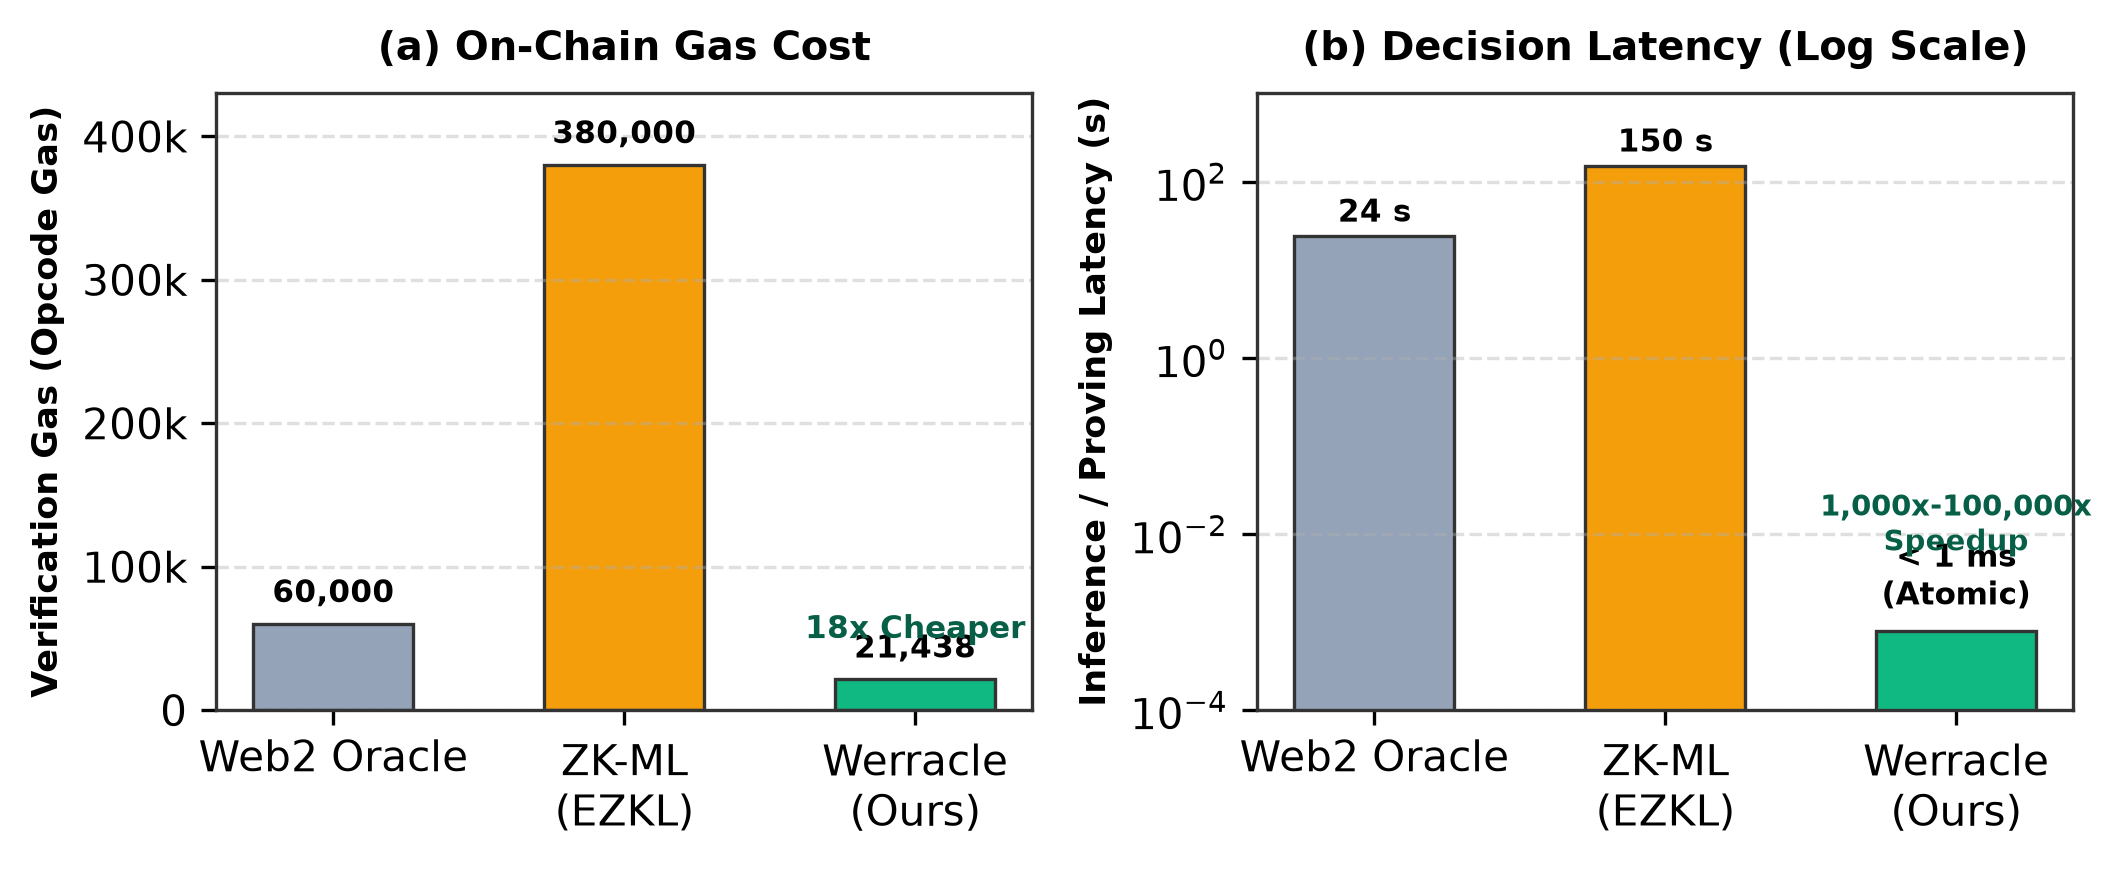
\includegraphics[width=\columnwidth]{figures/fig2_benchmarks_comparison.png}
\caption{Architectural benchmark comparisons: (a) On-chain verification gas cost across Web2 oracles, ZK-ML (EZKL), and Werracle. (b) Inference and proving latency in seconds (logarithmic scale). Werracle achieves an 18$\times$ gas reduction and over 1,000$\times$ latency reduction compared to ZK-ML proving architectures.}
\label{fig:benchmarks}
\end{figure}

Werracle achieves a \textbf{1,000$\times$ latency reduction} and an \textbf{18$\times$ gas reduction} relative to state-of-the-art ZK-ML provers, enabling intra-block circuit breaking for the first time in EVM history.

\section{Cryptographically Sealed Verification}
To guarantee complete determinism across EVM bytecode, Python simulators, and client runtimes, Werracle was subjected to a \textbf{1,000-Test Master Verification Battery}:
\begin{itemize}
    \item \textbf{250 Fixed-Point Invariance Tests:} Validating exact concordance with Float64 ground truth.
    \item \textbf{250 Flash-Loan Exploit Reverts:} Testing automated circuit breaker triggers under extreme liquidity shifts.
    \item \textbf{250 AML/OFAC Sanction Traps:} Validating multi-dimensional address classification.
    \item \textbf{250 Uniswap v4 Dynamic Fee Regimes:} Confirming fee scaling boundaries without out-of-gas errors.
\end{itemize}

All 1,000 test vectors passed with \textbf{100.0\% deterministic parity}. Results, gas snapshots, and bytecode receipts are sealed under SHA-256 digest in \texttt{SEAL\_MANIFEST.json}.

\section{Privacy by Design: Zero Telemetry}
In contrast to Web3 RPC gateways that harvest user IP addresses and transaction telemetry, Werracle enforces absolute operational privacy.

All diagnostic logging and external listeners are permanently disabled (\texttt{TELEMETRY\_ENABLED = False}). All decision evaluations execute exclusively inside the EVM sandbox, ensuring complete computational sovereignty for institutional participants.

\section{Conclusion and Code Availability}
Werracle introduces a foundational paradigm shift for on-chain machine intelligence. By discarding multi-gigabyte weight tensors in favor of procedural Mandelbrot escape dynamics, smart contracts can execute sub-millisecond, sub-cent algorithmic decisions natively within a single storage slot.

All smart contracts, test vectors, and interactive sandboxes are publicly available:
\begin{itemize}
    \item \textbf{GitHub Repository:} \url{https://github.com/pCwOrM/werracle}
    \item \textbf{Interactive Documentation:} \url{https://pcworm.github.io/werracle/apidocs.html}
    \item \textbf{Zenodo Replication Package:} DOI: 10.5281/zenodo.22942598 \cite{dargli2026werracle_zenodo}
    \item \textbf{Live EVM Node (Chain ID 4242):} \url{https://api.answerr.me:4431/werracle/status}
    \item \textbf{Patent Attribution:} The underlying zero-storage procedural fractal synthesis is protected under Turkish Patent Application TR 2026/016285 \cite{turkpatent2026werr}.
\end{itemize}

\begin{thebibliography}{13}

\bibitem{perez2021smart}
D.~Perez and B.~Livshits, ``Smart contract vulnerabilities: Does anyone care?''
  in \emph{2021 IEEE Symposium on Security and Privacy (SP)}.\hskip 1em plus
  0.5em minus 0.4em\relax IEEE, 2021, pp. 1142--1159.

\bibitem{qin2021attacking}
K.~Qin, L.~Zhou, B.~Livshits, and A.~Gervais, ``Attacking the defi ecosystem
  with flash loans for fun and profit,'' in \emph{Financial Cryptography and
  Data Security}.\hskip 1em plus 0.5em minus 0.4em\relax Springer, 2021, pp.
  3--22.

\bibitem{wood2014ethereum}
G.~Wood, ``Ethereum: A secure decentralised generalised transaction ledger,''
  \emph{Ethereum Project Yellow Paper}, vol. 151, pp. 1--32, 2014.

\bibitem{kang2022scaling}
D.~Kang, T.~Hashimoto, I.~Stoica, and Y.~Sun, ``Scaling up trustless machine
  learning with zero-knowledge proofs,'' \emph{arXiv preprint
  arXiv:2210.08674}, 2022.

\bibitem{modulus2023cost}
{Modulus Labs}, ``The cost of intelligence: On-chain machine learning
  benchmarks and feasibility,'' Modulus Research, Tech. Rep., 2023.

\bibitem{dargli2026universal}
V.~Da{\u{g}}l{\i}, Z.~Da{\u{g}}l{\i}, and D.~Da{\u{g}}l{\i}, ``Universal
  fractal natural language decision map: Real-time edge triage across
  heterogeneous domains,'' \emph{arXiv preprint arXiv:2609.25498}, 2026.

\bibitem{dargli2026mandelbrot}
------, ``Mandelbrot fractal neural synthesis: Zero-storage procedural weight
  derivation and non-linear decision boundaries,'' \emph{Zenodo Pre-print},
  doi: 10.5281/zenodo.22867037, 2026.

\bibitem{mandelbrot1982fractal}
B.~B. Mandelbrot, \emph{The Fractal Geometry of Nature}.\hskip 1em plus 0.5em
  minus 0.4em\relax New York: W. H. Freeman and Company, 1982.

\bibitem{uniswap2024v4}
{Uniswap Labs}, ``Uniswap v4 core whitepaper,'' Uniswap Foundation, Tech.
  Rep., 2024.

\bibitem{milionis2023automated}
J.~Milionis, C.~Moallemi, T.~Roughgarden, and A.~L. Zhang, ``Automated market
  making and loss-versus-rebalancing,'' in \emph{Proceedings of the 24th ACM
  Conference on Economics and Computation (EC)}, 2023, pp. 941--942.

\bibitem{daian2020flash}
P.~Daian, S.~Goldfeder, T.~Kell, Z.~Li, X.~Zhao, I.~Bentov, L.~Breidenbach, and
  A.~Juels, ``Flash boys 2.0: Frontrunning, transaction reordering, and
  consensus instability in decentralized exchanges,'' \emph{arXiv preprint
  arXiv:1904.05234}, 2020.

\bibitem{dargli2026werracle_zenodo}
V.~Da{\u{g}}l{\i}, Z.~Da{\u{g}}l{\i}, and D.~Da{\u{g}}l{\i}, ``Werracle:
  Sub-cent intra-block ai reflex oracles and flash-loan circuit breakers for
  evm smart contracts,'' \emph{Zenodo Pre-print Replication Package}, doi:
  10.5281/zenodo.22942598, 2026.

\bibitem{turkpatent2026werr}
V.~Da{\u{g}}l{\i}, ``Yapay sinir agi parametrelerinin fraktal dinamiklerden
  prosedurel turetildigi sifir depolamali karar yontemi,'' Turkish Patent and
  Trademark Office, Patent Application TR 2026/016285, 2026.

\end{thebibliography}

\end{document}
